\section{Experiment Evaluation}

To validate the effectiveness of our approach, we simulated various attacks on 100 critical system processes, resulting in 10 APT (Advanced Persistent Threat) attack scenarios. We then evaluated our method based on the following five aspects:

\begin{itemize}
    \item \textbf{Q1.} How well does our method work, and does it achieve a low false-positive rate? ((§~\ref{sec-effective})
    \item \textbf{Q2.} What is the time it takes for our method to construct a profile for each process? What is the most time-consuming step in the three-step process profile creation? (§~\ref{sec-eff})
    \item \textbf{Q3.} How does the behavior diverge based on LLM, and how does the verification step optimize the outcome? (§~\ref{sec-ab-study})
    \item \textbf{Q4.} How can we validate the accuracy of these explanations using our method? (§~\ref{sec-explanation-val})
    \item \textbf{Q5.} Is it common for real-world APT attacks to disguise their processes in various ways? (§~\ref{sec-real-world})
\end{itemize}
All experiments are performed on a server with Intel Xeon E5-2620 v4 CPUs @ 2.10GHz, 64 GB physical memory, and an NVIDIA Tesla V100 GPU. The OS is Ubuntu 16.04.3 LTS.


\subsection{Implementation}
We present important technical details in the implementation.

\subsubsection{System Auditing Collection}

While ProCon is engineered to handle inputs from both Linux and Windows systems, our evaluation predominantly emphasizes Windows events. This is largely due to the fact that our benign deployment environment is majorly comprised of Windows-based hosts, and a significant portion of sophisticated malware is specifically crafted for Windows platforms. To effectively gather provenance data from these systems, we turn to Sysmon, Windows' sophisticated log collection tool. By leveraging Sysmon's default settings, we ensure a thorough and exhaustive capture of system logs.

\subsubsection{Simulated Datasets}

% Apt攻击场景
% 常见的6种伪装的类型
% Process Masquerade
% Parent PID Spoofing
% Process Hollow
% Process Injection
% DLL Side-Loading
% Functional Masquerade 

% 不同节点类型的伪装
% 文件类型
% Dll

In forensic analysis, the lack of publicly available attack datasets and system logs is a common challenge. For example, the data released by DARPA's Transparent Computing program do not include audit logs generated during evaluation engagements and also lack explicit labels. 

To tackle the challenges, we approached the problem from three perspectives: enhancing stealthy attack coverage, simulating realistic APT scenarios, and accounting for previously unseen attack methodologies. 
For our simulations, we relied on well-known hacker utilities like Caldera, complemented by our bespoke C++ programs crafted to execute a spectrum of attack functionalities. This included strategies for Initial Access, Privilege Escalation, Information Gathering, Defense Evasion, and ensuring Persistence.


\textbf{Attack Datasets.}
\begin{itemize}
    \item  Stealthy attack coverage: We rank attacks into six categories based on their level of stealth. These categories, from the least to the most stealthy, are: Process Masquerade, Parent PID Spoofing, Process Hollow, Process Injection, DLL Side-Loading, and Functional Masquerade. For basic disguises like Process Masquerade, we've created our proprietary software designed for actions like maintaining persistence and gathering information. For more sophisticated techniques such as Process Injection and DLL Side-Loading, we design malicious DLLs to execute these actions.
    \item Realistic APT scenarios: To enhance the realism of our simulations, we crafted ten APT attack scenarios based on in-depth reports of real-world Advanced Persistent Threat (APT) activities, generating audit logs within a controlled testbed environment. The process of implementing these APT attacks was as follows: Drawing from the genuine APT reports, we selected the aforementioned six stealthy attack techniques. For each technique, based on the specific details outlined in the APT reports, we designed varying payloads (either in the form of DLLs or EXEs). Each payload was tailored with distinct malicious functionalities, such as information gathering or privilege escalation, to emulate the multifaceted nature of actual APT attacks.
    \item Unseen attack methodologies: To demonstrate that our attacks can detect unknown threats, we implemented a more stealth attack known as Functional Masquerade. This involves exploiting the normal functionalities of legitimate programs for malicious activities.
\end{itemize}

\textbf{Normal Datasets.}
Additionally, similar to previous work that constructs benign system events, we emulate diverse normal user activities on the same machine during each attack execution to the best of our ability. More specifically, we manually generate various benign user activities like browsing different websites, executing different applications (e.g., reading emails, downloading attachments), and connecting to other hosts.

\textbf{Label.}
With our full knowledge of attack workflow, we manually label the ground truth of interactions through their relations to attacks.


\subsubsection{Process Classification}

In order to construct a comprehensive analysis framework, we strategically selected 100 pivotal processes for examination. The selection criteria encompassed multiple dimensions, including: 1) Core system processes that are integral to system functionality; 2) Processes highly associated with security mechanisms; and 3) Processes commonly utilized by system administrators. Additionally, we integrated an assessment of processes that are frequently targeted in cyber-attacks, based on statistical analysis derived from MITRE's official website as shown in Figure~\ref{fig-process}

\begin{figure}[h]
    \centering
      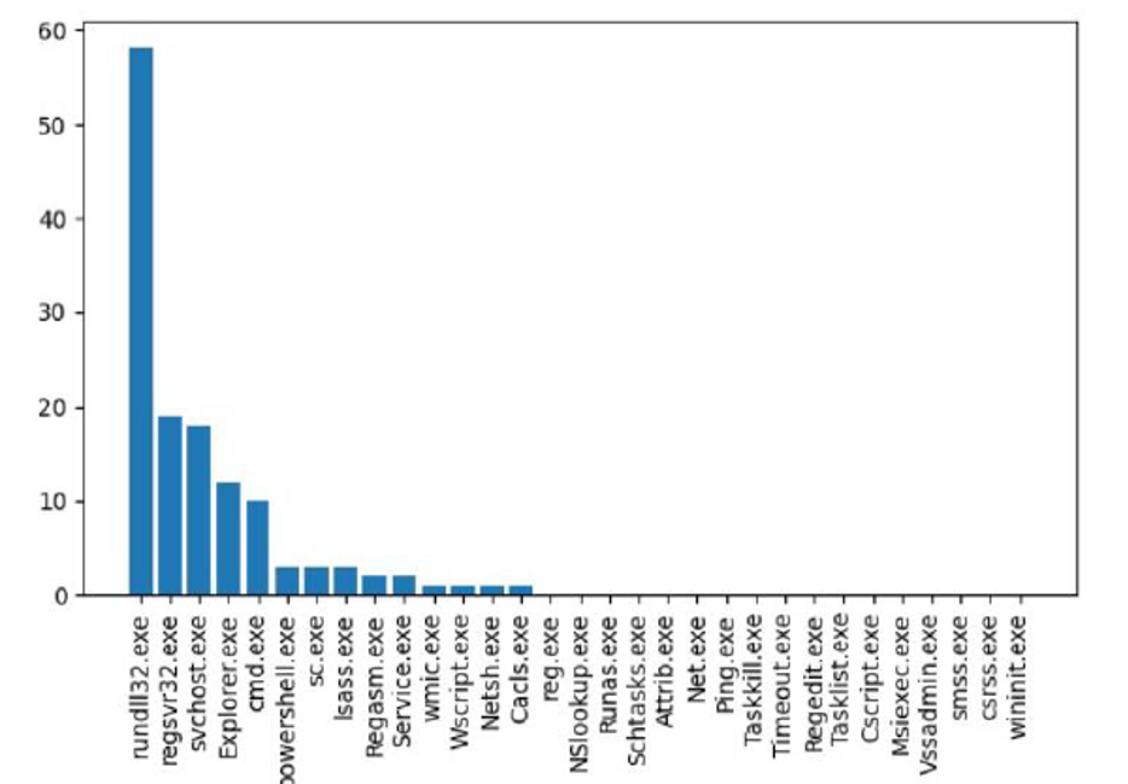
\includegraphics[width=0.49\textwidth]{figs/process.png}
    \caption{Comparison of attack frequencies for different processes based on the official MITRE website.}
    \label{fig-process}
\end{figure}

% \begin{table*}[h!]
%     \centering
%     \begin{tabularx}{\textwidth}{|l|l|X|}
%     \hline
%     \textbf{Process} & \textbf{Categories} & \textbf{Description} \\
%     \hline
%     svchost.exe & wlidsvc & Microsoft Account Sign-in Assistant which enables user to sign-in through Microsoft account identity services. \\
%     \cline{2-3}
%     & WaaSMedicSvc & Windows Update Medic Service fixes any damages suffered by the Windows Update component. \\
%     \cline{2-3}
%     & wuauserv & Windows Update Service enables the detection, download, and installation of updates for Windows. \\
%     \cline{2-3}
%     & ClipSVC & Client License Service provides infrastructure support for the Microsoft Store. \\
%     \cline{2-3}
%     & BITS & Background Intelligent Transfer Service downloads files from or uploads files to HTTP web servers and SMB file shares. \\
%     \hline
%     rundll32.exe & DispatchAPICall & Call an API function within a DLL file mainly used for executing system commands. \\
%     \cline{2-3}
%     & ShellRefresh & Refresh the Windows Universal App Package cache to resolve issues related to the installation, update, or removal of Universal Windows Platform (UWP) apps. \\
%     \cline{2-3}
%      & StateRepositoryDoMaintenanceTasks & Perform maintenance tasks on the Windows state repository to resolve issues related to the state repository. \\
%     \cline{2-3}
%     & PcaPatchSdbTask & Performing patching or updating system software or drivers \\
%     \hline
%     \end{tabularx}
%     \caption{Processes and Descriptions}
%     \label{tab:process}
% \end{table*}


\begin{table}[h]
\centering
\begin{tabular}{|c|c|c|c}
\hline
 & Precision & Recall & F1-Score \\
\hline
Process Masquerade & & &  \\
\hline
Parent PID Spoofing & & &  \\
\hline
Process Hollow & & &  \\
\hline
Dll Process Injection & & &  \\
\hline
DLL Side-Loading & & &  \\
\hline
Functional Masquerade  & & &  \\
\hline
\end{tabular}
\caption{Your table caption here}
\label{tab:my_label}
\end{table}

Descriptions of various processes can be found in the Appendix. Here, we highlight the two most common processes: svchost.exe and rundll32.exe as shown in Table~\ref{tab:process}.

\textbf{Svchost.exe processes}. svchost.exe is a Windows system program that hosts wide range of hardware and OS related services daemons in the background whose behaviors are determined by command line arguments, which load different library (e.g., .dll) files. Due to the svchost.exe’s persistent presence and its well-trusted nature, adversaries often impersonate svchost.exe to launch their attack payloads. Therefore, in addition to the benign program classification task using svchost.exe, we also exercised an anomaly detection task to distinguish between benign and malicious svchost.exe instances. Detailed list of svchost.exe programs invoked with different command line arguments are listed in Table 4 alongside their brief descriptions.

\textbf{Rundll32.exe processes}. rundll32.exe hosts specific functions exported from library (e.g., .dll) files. While similar to svchost.exe, rundll32.exe is more easily exploited, as an attacker can write their own .dll to be loaded by rundll32.exe. Security incident reports and research rank rundll32.exe as one of the most favored targets for malware impersonation because it can be used to embed malicious .dlls into the target’s address space using a legitimate host program. We conducted two sets of evaluations for rundll32.exe: program classification for benign rundll32.exe applications and anomaly detection for malware samples that impersonate rundll32.exe. The different categories of tasks include calling API functions within a .dll to execute system commands, refreshing Windows Universal App Package cache, performing maintenance tasks on the Windows state repository, and updating and patching system software or driver. These tasks can help resolve various issues related to system settings, installation and removal of UWP apps, and performance optimization. A detailed list of rundll32.exe programs that load different .dll are listed in Table 4 alongside their brief descriptions.


\subsection{Effectiveness}
\label{sec-effective}
In this study, we assess the detection efficacy of ProCon through the use of precision, recall, F1-score, and accuracy metrics. More specifically, precision measures correctly detected threats against predicted threats; recall measures correctly detected threats against ground-truth threats; and F1score calculates the harmonic mean of the precision and recall.

\subsubsection{Evaluation on Attack for Various Processes}
We initiate stealthy attacks on 100 processes and collect the attack logs. How does our method fare in terms of false negatives? We'll use a case study to analyze how our method detects malicious activities.

As mentioned in the previous section, we evaluate our approach from three distinct dimensions, with one primary focus on the coverage of attack detection. For this assessment, we systematically executed six types of stealthy attacks on 100 commonly encountered processes. Each attack payload was designed to implement one of six functionalities, such as information gathering and privilege escalation. This resulted in a comprehensive testing scenario involving 3,600 attack detection tasks. The outcomes of our method's detection are depicted in the following figure.

Subsequently, we delve into a detailed analysis to identify the reasons behind any false positives and false negatives produced by our approach.

\textbf{Analysis of False Positives.}

\textbf{Analysis of False Negatives.}

\subsubsection{Evaluation on Normal Workloads}
In 100 processes, we stimulate benign behaviors triggered by LLM and collect the corresponding logs. How does our method perform in terms of false positives? some case study will help understand why our method can achieve low false positives.

\subsubsection{Evaluation on APT scenarios}
we construct 10 APT attack scenarios by combining single attack behavior and compare our method against four state-of-the-art techniques. By analyzing cases where current methods exhibit false positives, we aim to explain why these methods might produce false positives.

\textbf{ProvDetector.}
Among the methods most analogous to ours is "ProvDetector." 
This approach \cite{wang2020you} aims to identify malware by analyzing the provenance graph. It transforms paths within the graph into embedded representations and then employs the Local Outlier Factor technique for malware detection.
We drew insights from results based on event investigation to evaluate the efficacy of our method against ProvDetector.

\textbf{ThreaTrace.}
ThreaTrace \cite{wang2022threatrace} constructs a unique model for each node type within a provenance graph, aiming to identify anomalies at the node level. Consequently, our comparison with ThreaTrace centers around the results derived from entity (or node) based detection.

\textbf{ATLAS.}
ATLAS \cite{alsaheel2021atlas} derives both attack and non-attack sequences from
graphs and uses sequence models to discern attack patterns,
recognizing that distinct attacks might exhibit analogous ab-
stract strategies, irrespective of exploited vulnerabilities and
executed payloads
We will juxtapose our results, both from the perspectives of entity (nodes) and event (edges), against those produced by ATLAS.

\textbf{Shadewatcher.}
SHADEWATCHER \cite{zengy2022shadewatcher} utilizes knowledge graph embeddings to represent each node and edge. Originally tailored for information flow, we've adapted the method to suit our comparative analysis. Focusing on process nodes, we center our representation on a process and its 1st to 2nd order neighbors, forming a subgraph. The rest of the components remain consistent with the original methodology.


\begin{table*}[htbp]
\centering
\caption{Your caption here}
\begin{tabularx}{\textwidth}{|c|c|c|c|c|}
\hline
\textbf{Attack ID} & \textbf{\#Attack Entity} & \textbf{\#Non-attack Entity} & \textbf{\#Attack Event} & \textbf{\#Non-attack Event} \\
\hline
S-1 & 22 & 7,445 & 12 & 34,008  \\
S-2 & ... & ... & ... & ...  \\
... & ... & ... & ... & ...  \\
M-6 & 42 & 19,580 & 4,598 & 90,467  \\
\hline
Avg. & 28 & 20,051 & 17,341 & 275,796 \\
\hline
\end{tabularx}
\end{table*}


\subsection{Efficiency}
\label{sec-eff}
What is the time it takes for our method to construct a profile for each process? What is the most time-consuming step in the three-step process profile creation?

\subsection{Ablation Study}
\label{sec-ab-study}

What is the time it takes for our method to construct a profile for each process? What is the most time-consuming step in the three-step process profile creation?
We conduct an ablation study to understand the contributions of the three key modules: Process Tree Construction Module, Command Execution Module, and Constraint Extraction Module, to the overall performance of ProCon GPT. We present three distinct variants for our analysis:

\begin{itemize}
    \item ProCon GPT-NO-tree-construction: In this variant, the Process Tree Construction Module is deactivated, resulting in all data being fed directly into the system without any hierarchical organization.
    \item Procon GPT-NO-Verification: The Constraint Extraction Module is disabled in this variant. Instead of using the Process Tree Construction approach, this model leverages the same techniques as those employed with LLMs for penetration testing, as outlined in the Exploratory Study.
\end{itemize}

\subsection{Explanation Validation}
\label{sec-explanation-val}
How can we validate the accuracy of these explanations using our method?
Our approach seamlessly integrates detection and interpretation. In the following sections, we will delve into how our method elucidates attack behaviors, thereby assisting security analysts in rapidly verifying and responding to threats.

\subsection{Real-world Validation}
\label{sec-real-world}
Is it common for real-world APT attacks to disguise their processes in various ways?

